
\noindent\textbf{Dataset.}
We conduct experiments on five real-world datasets, including the \textit{Reddit}, \textit{Wiki}, \textit{MOOC}, \textit{LastFM} datasets that are used in~\cite{kumar2019predicting} and the \textit{GDELT} dataset\footnote{The \textit{GDELT} dataset used in our paper is a sub-sampled version because the original dataset is too big to fit into memory for single-machine training. In practice, we keep $1$ temporal link per $100$ continuous temporal link.} which is introduced in~\cite{zhou2022tgl}.
Besides, since \textit{GDELT} is the only dataset with both node and link features, we create its two variants to understand the effect of training data on model performance: \textit{GDELT-e} removes the link feature from \textit{GDELT} and keep the node feature and link timestamps, \textit{GDELT-ne} removes both the link and edge features from \textit{GDELT} and only keep the link timestamps.
For each dataset, we use the same $70\%/15\%/15\%$ chronological splits for the train/validation/test sets as existing works.
The detailed dataset statistics are summarized in Appendix~\ref{section:dataset}. 

\noindent\textbf{Baselines.}
We compare baselines that are introduced in Section~\ref{section:related_works}. 
% For a fair comparison, we implement \our and compare with baselines under the temporal graph learning framework~\cite{zhou2022tgl}. 
Besides, we create two variants to better understand how node- and link-information contribute to our results, where \oure-L is only using link-encoder and \oure-N is only using node-encoder.
We conduct experiments under the transductive learning setting and use average precision for evaluation.
The detailed model configuration, training and evaluation process are summarized in Appendix~\ref{section:model_config_train_eval_process}.
Due to the space limit, more experiment results on using \emph{Recall@K, MRR, and AUC} as the evaluation metrics, comparison on \emph{wall-clock time} and \emph{number of parameters} are deferred to Appendix~\ref{section:more_experiment_results}

\noindent\textbf{Outline.} We first compare \our with baselines in Section~\ref{section:empirical_results} then highlight the three key factors that contribute to the success of \our in Section~\ref{section:time_encoder}, Section~\ref{section:expressive_power}, and Section~\ref{section:data_alignment}.

% \begin{table}[t]
% \caption{Comparison on the average precision score for link prediction. } % and  Hits$@$K 
% \label{table:average_precision}
% \vspace{-3mm}
% \centering
% \scalebox{9}{
% \begin{tabular}{ l r  c c  c  c| c c }
% \hline\hline
%       & & Reddit & Wiki & MOOC & LastFM & GDELT (-) & GDELT (+)\\ \hline\hline
% JODIE & (RNN) & $9930$ & $9881$ & $9916$ & $6751$ & $9713$ & $9696$ \\ 
% DySAT &(SAM) & $9852$ & $9671$ & $9882$ & $7640$ & $8247$ & $9725$ \\ 
% TGAT  &(SAM) & $9966$ & $9775$ & $9843$ & $5477$ & $8430$ & $9696$ \\ 
% TGN   & (RNN+SAM) & $9980$ & $9955$ & $9962$ & $8223$ & $9713$ & $9604$ \\ \hline
% \our & (Time only) & $9984$ & $9970$ & $9981$ & $9374$ & $9614$ & $9614$ \\ 
% \our & (Structure only) & $9924$ & $9033$ & $9735$ & $6380$ & $9600$ & $9600$\\ 
% \our & (Time + Structure) & $\textcolor{red}{9993}$ & $\textcolor{red}{9985}$ & $\textcolor{red}{9991}$ &  $\textcolor{red}{9631}$ & $\textcolor{red}{9839}$ & \textcolor{red}{9822}\\ \hline
% JODIE & (Fixed time-encoder)     & 9976 & 9900 & 9917 & 7989 & & 9696    \\ 
% TGAT & (Fixed time-encoder)     & 9948 & 9855 & 9933 & 7626 & & 9628    \\
% TGN & (Fixed time-encoder)     & 9983 & 9954 & 9962 & 8758 & & 9734    \\ 
% \hline\hline
% \end{tabular}}
% \end{table}



\begin{table}[t]
\caption{Comparison on the average precision score for link prediction. \our uses one-hot node encoding for datasets without node features (marked by $\natural$). For each dataset, we indicate whether we have the corresponding feature (``L'' link features, ``N'' node features, and ``T'' link timestamps). 
\textcolor{red}{Red} is the best score, \textcolor{blue}{Blue} is the best score excluding \our and its variants.
% and the average number of temporal links per node in the dataset.
}  % and  Hits$@$K , baselines either uses link features and time features (marked by $$) or uses random features  (marked by $$) as node features  
\label{table:average_precision}
\vspace{-3mm}
\centering\setlength{\tabcolsep}{1.7mm}
\centering
\scalebox{0.75}{
\begin{tabular}{ l cccc ccc}
\hline\hline
       & Reddit & Wiki & MOOC & LastFM & GDELT & GDELT-ne & GDELT-e \\
       & L, T & L, T & T & T & L, N, T & T & N, T \\
    %   & Node / links & 11K/7M & 9K/6M & 7K/4M & 2K/1.3M & 9K/2M & 9K/2M & 9K/2M \\
    %   & Links per node & 61.2 & 17.1 & 57.6 & 653.1 & 216.6 & 216.6 & 216.6 \\ 
      \hline\hline
JODIE & $99.30 \pm 0.01$ & $98.81 \pm 0.01$ & $99.16 \pm 0.01$ & $67.51 \pm 0.87$ & $98.27 \pm 0.02$ & $97.13 \pm 0.02$ & $96.96 \pm 0.02$ \\ 
DySAT & $98.52 \pm 0.01$ & $96.71 \pm 0.02$ & $98.82 \pm 0.02$ & $76.40 \pm 0.77$ & $\textcolor{blue}{98.52} \pm 0.02$ & $82.47 \pm 0.13$ & $\textcolor{blue}{97.25} \pm 0.02$\\ 
TGAT  &  $99.66 \pm 0.01$ & $97.75 \pm 0.02$ & $98.43 \pm 0.01$ & $54.77 \pm 1.01$ & $98.25 \pm 0.02$ & $84.30 \pm 0.10$ & $96.96 \pm 0.02$ \\ 
TGN   &  $\textcolor{blue}{99.80} \pm 0.01$ & $\textcolor{blue}{99.55} \pm 0.01$ & $\textcolor{blue}{99.62} \pm 0.01$ & $\textcolor{blue}{82.23} \pm 0.50$ & $98.15 \pm 0.02$ & $97.13 \pm 0.02$ & $96.04 \pm 0.02$ \\ \hline
CAWs-mean& $98.43 \pm 0.02$ & $97.72 \pm0.03$ & $62.99\pm0.87$ & $76.35\pm 0.08$ & $95.11 \pm 0.12$ & $69.20 \pm 0.10$ & $91.72 \pm 0.19$\\
CAWs-attn& $98.51 \pm 0.02$ & $97.95 \pm0.03$ & $63.07\pm0.82$ & $76.31 \pm 0.10$ & $95.06 \pm 0.11 $ & $69.54 \pm 0.19$ & $91.54 \pm 0.22$ \\
% TGN-MeTA & $99.08 \pm 0.1$ & $99.08 \pm 0.1$ & $92.03 \pm 0.3$ & & & \\
% DyRep-MeTA & $98.62 \pm 0.1$ & $95.63 \pm 0.2$ & $84.18 \pm 0.3$ & & & \\
TGSRec & $95.21 \pm 0.08$ & $91.64 \pm 0.12$ & $83.62 \pm 0.34$ & $76.91 \pm 0.87$ & $97.03 \pm 0.61$ & $97.03 \pm 0.61$ & $97.03 \pm 0.61$ \\
APAN & $99.24 \pm 0.02$ & $98.14 \pm 0.01$ & $98.70 \pm 0.98$ & $69.39 \pm 0.81$ & $95.96 \pm 0.10$ & $\textcolor{blue}{97.38} \pm0.23$ & $96.77 \pm 0.18$\\ \hline 
\oure-L &  $99.84 \pm 0.01$ & $99.70 \pm 0.01$ & $99.81 \pm 0.01$ & $95.50 \pm 0.03$ & $\textcolor{red}{98.99} \pm 0.02$ & $96.14 \pm 0.02$ & $\textcolor{red}{98.99} \pm 0.02$ \\ 
\oure-N &  $99.24 \pm 0.01^\natural$ & $90.33 \pm 0.01^\natural$ & $97.35 \pm 0.02^\natural$ & $63.80 \pm 0.03^\natural$ & $94.44 \pm 0.02$ & $96.00 \pm 0.02^\natural$ & $98.81 \pm 0.02^\natural$ \\ 
\our &  $\textcolor{red}{99.93} \pm 0.01^\natural$ & $\textcolor{red}{99.85} \pm 0.01^\natural$ & $\textcolor{red}{99.91} \pm 0.01^\natural$ &  $\textcolor{red}{96.31} \pm 0.02^\natural$ & $98.89 \pm 0.02$ & $\textcolor{red}{98.39} \pm 0.02^\natural$ & $98.22 \pm 0.02^\natural$ \\ 
% JODIE & (Fixed time-encoder)     & 9976 & 9900 & 9917 & 7989 & & 9696    \\ 
% TGAT & (Fixed time-encoder)     & 9948 & 9855 & 9933 & 7626 & & 9628    \\
% TGN & (Fixed time-encoder)     & 9983 & 9954 & 9962 & 8758 & & 9734    \\ 
\hline\hline
\end{tabular}}
\vspace{-4mm}
\end{table}




\subsection{Main empirical results.} \label{section:empirical_results}


\noindent\textbf{\our achieves outstanding performance.}
We compare the average precision score with baselines in Table~\ref{table:average_precision}. We have the following observations: 
\circled{1} \our outperforms all baselines on all datasets. 
% In particular, \our attains more than $1\%$ gain over all baselines on the \textit{LastFM}, \textit{GDELT-ne}, and \textit{GDELT-e} datasets, attains around $2\%$ gain over non-RNN methods \textit{DySAT} and \textit{TGAT} on the \textit{Wiki} dataset, and attains more than $11\%$ gain over non-RNN methods \textit{DySAT} and \textit{TGAT} on the \textit{GDELT-ne} dataset. 
The experiment results provide sufficient support on our argument that neither RNN nor SAM is necessary for temporal graph link prediction.
\circled{2} According to the performance of \oure-L on datasets only have link timestamp information (\textit{MOOC}, \textit{LastFM}, and \textit{GDELT-ne}), we know that our time-encoding function could successfully pre-process each timestamp into a meaningful vector. In fact,  we will show later in Section~\ref{section:time_encoder} that our time-encoding function is more preferred than baselines' trainable version.
    % \item Datasets with greater temporal links per node, e.g., \textit{LastFM} and \textit{GDELT}, are more challenging to learn.  
\circled{3} By comparing the performance \oure-N and \our on \textit{Wiki}, \textit{MOOC}, and \textit{LastFM} datasets, we know that node-encoder alone is not enough to achieve a good performance. However, it provides useful information that could benefit the link-encoder.
\circled{4} By comparing the performance of \oure-N on \textit{GDELT} and \textit{GDELT-ne}, we observe that using one-hot encoding outperforms using node features. This also shows the importance of node identity information because one-hot encoding only captures such information.
\circled{5} More complicated methods (e.g., CAWs, TGSRec, and DDGCL) do not perform well when using the default hyper-parameters\footnote{In fact, we tried different hyper-parameters based on their default values, but the results are similar.}, which is understandable because these methods have more components with an excessive amount of hyper-parameters to tune.

\begin{figure}[h]
\centering
\begin{subfigure}{0.32\textwidth}
    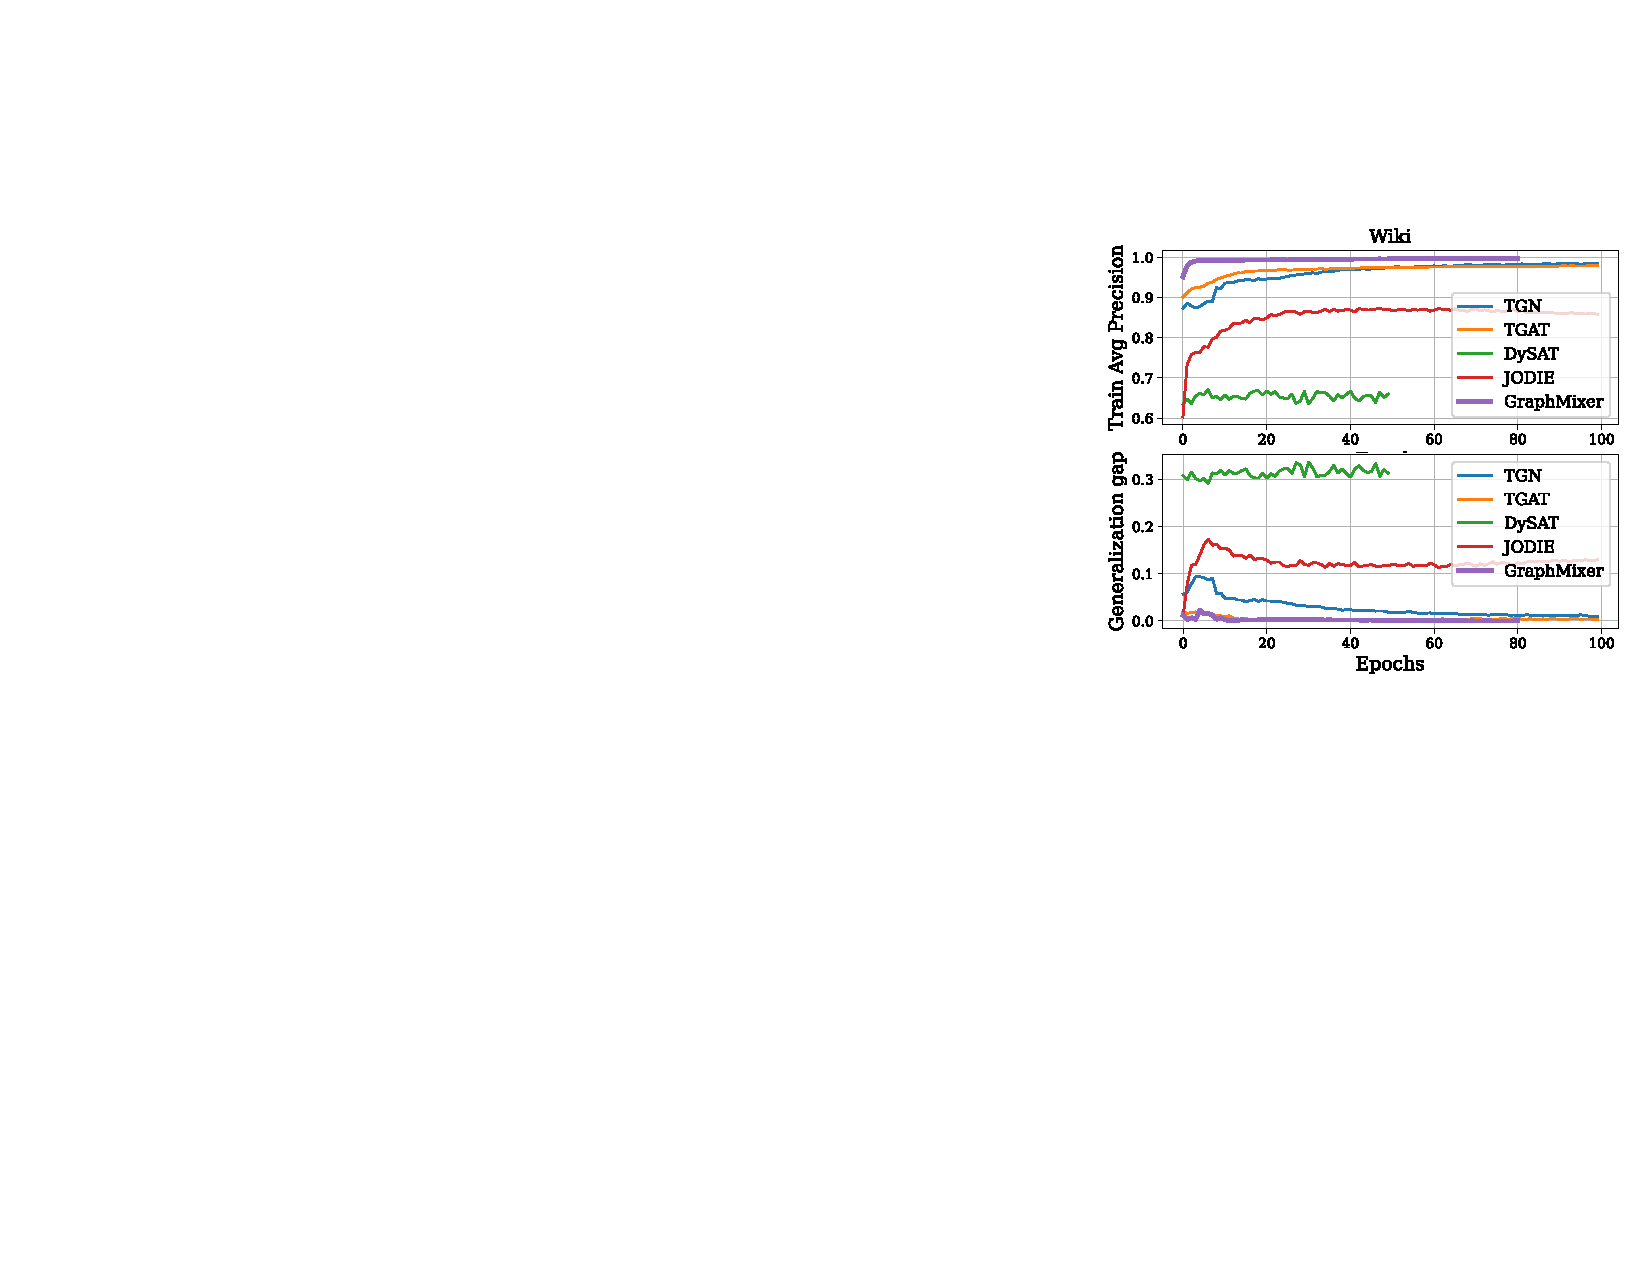
\includegraphics[width=\textwidth,height=2.5cm,height=3.5cm]{figures/train_extra/wiki_train_extra.pdf}
    \vspace{-6.5mm}
    % \caption{Evaluation average precision}
    % \label{fig:first}
\end{subfigure}
\hspace{0cm}
\begin{subfigure}{0.32\textwidth}
    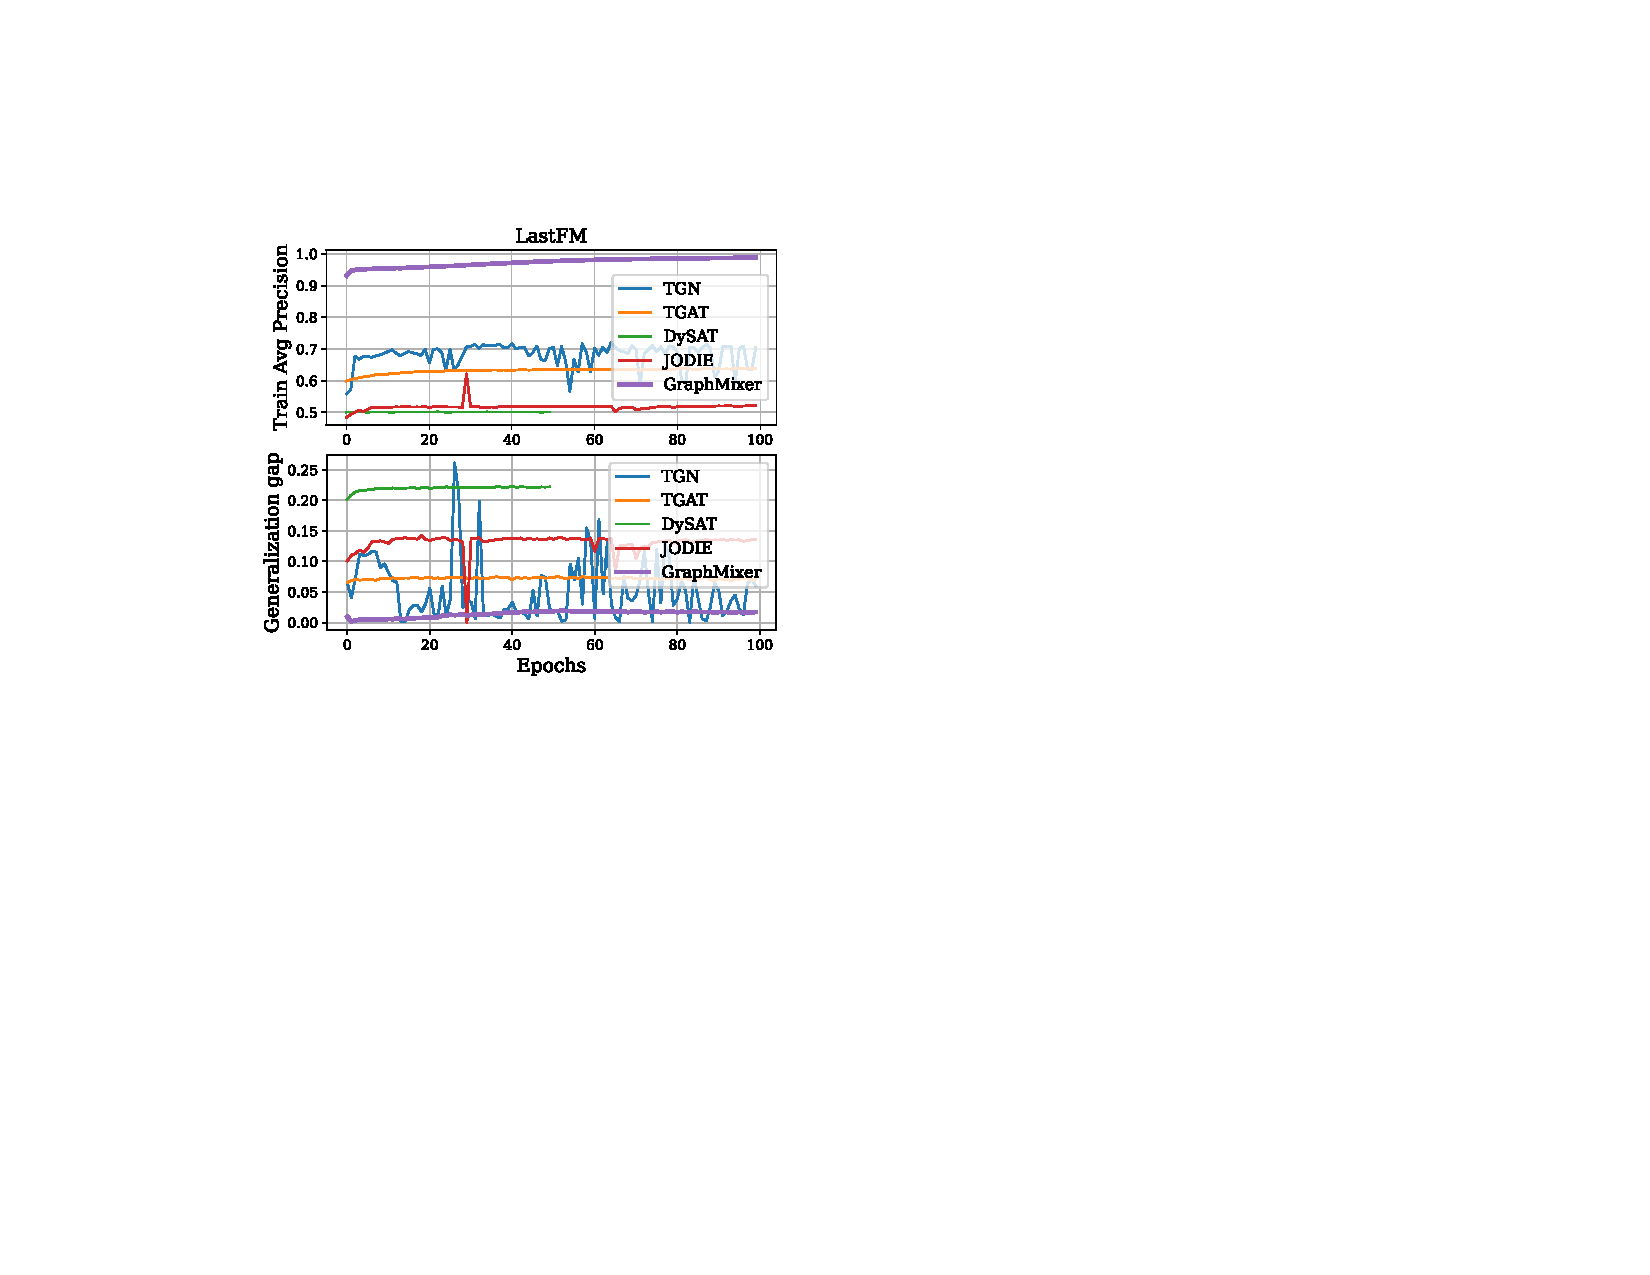
\includegraphics[width=\textwidth,height=2.5cm,height=3.5cm]{figures/train_extra/lastfm_train_extra.pdf}
    \vspace{-6.5mm}
    % \caption{Train average precision}
    % \label{fig:second}
\end{subfigure}
\hspace{0cm}
\begin{subfigure}{0.32\textwidth}
    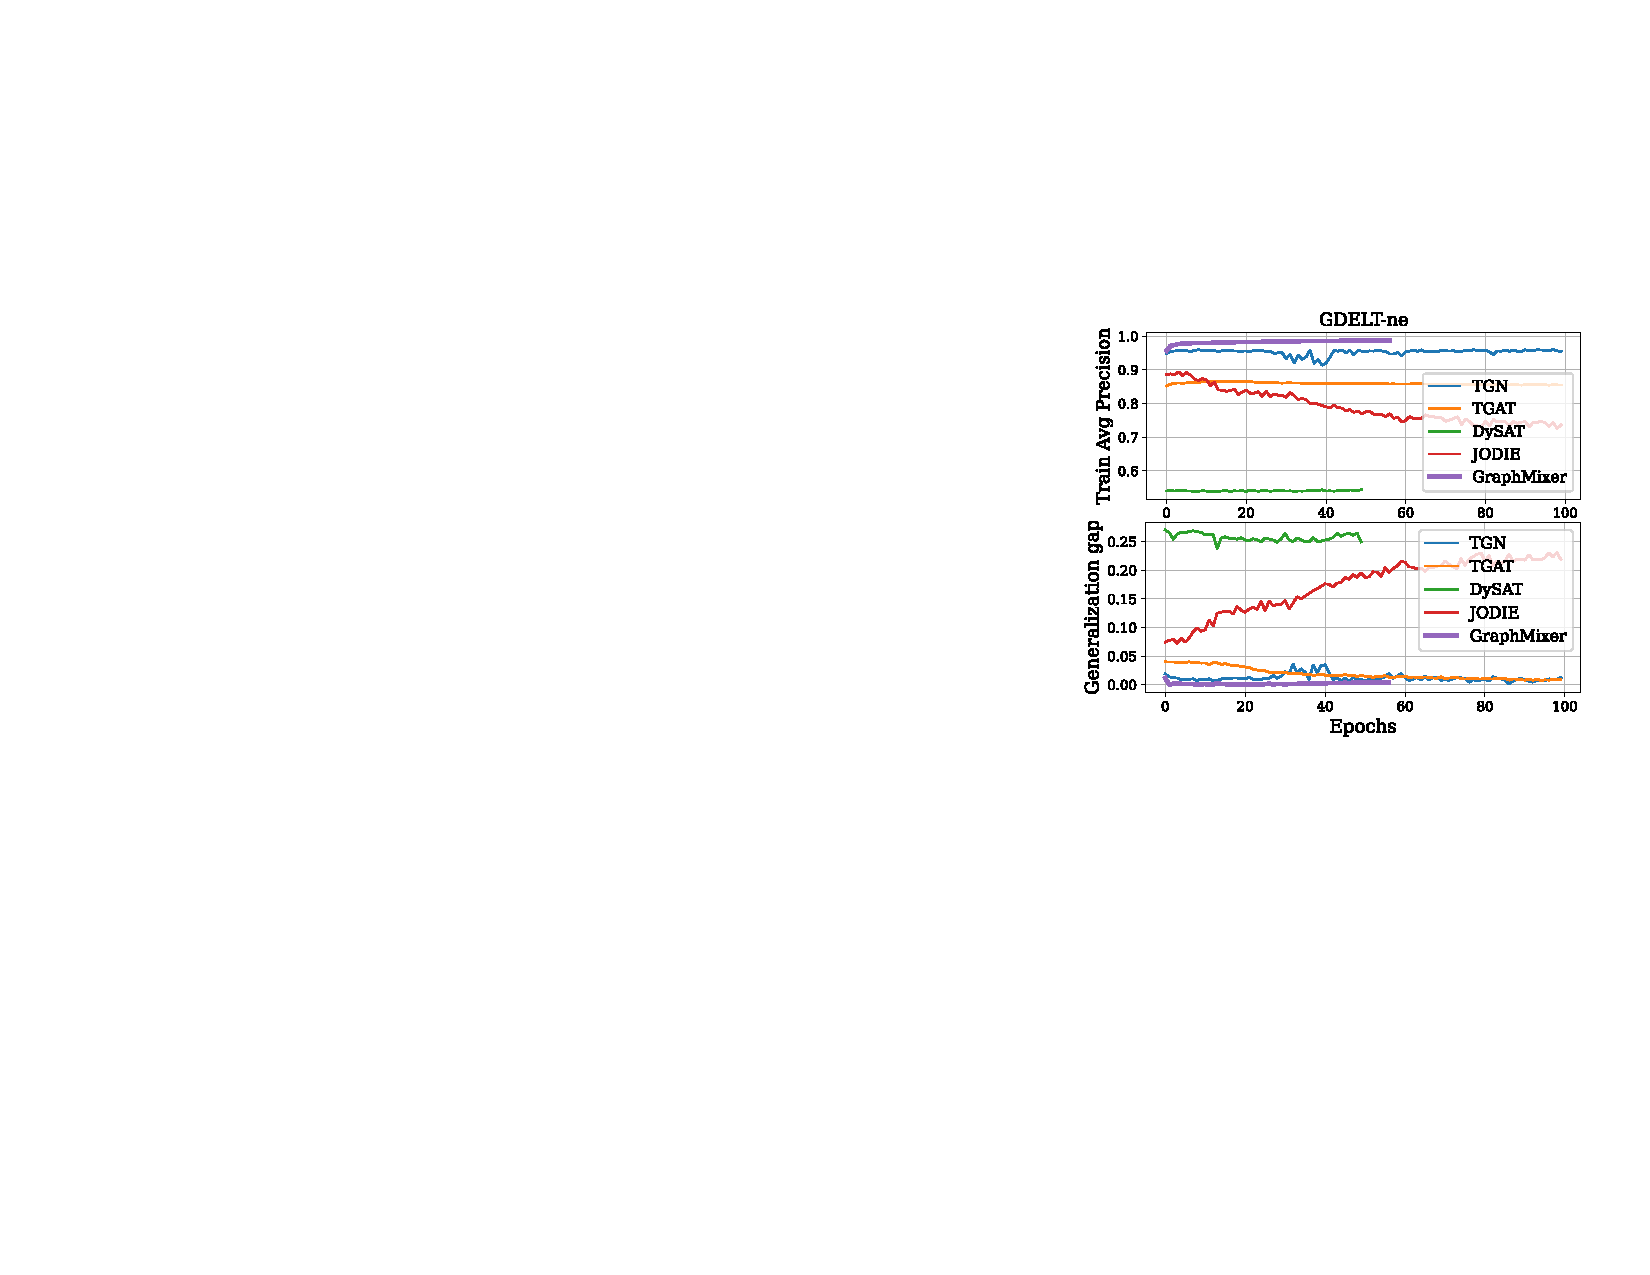
\includegraphics[width=\textwidth,height=2.5cm,height=3.5cm]{figures/train_extra/gdelt_ne_train_extra.pdf}
    \vspace{-6.5mm}
    % \caption{Generalization gap}
\end{subfigure}
\vspace{-1mm}
\caption{Comparison on the training set average precision and generalization gap for the first $100$ training epochs. Results on other datasets can be found in Figure~\ref{fig:train_extra_reddit_mooc_gdelt_e}.}
\label{fig:train_extra_wiki_lastfm_gdelt_ne}
\vspace{-2mm}
\end{figure}

\noindent\textbf{\our enjoys better convergence and generalization ability.}
To better understand the model performance, we take a closer look at the dynamic of training accuracy and the generalization gap (the absolute difference between training and evaluation score).
The results are reported in Figure~\ref{fig:train_extra_wiki_lastfm_gdelt_ne} and Figure~\ref{fig:train_extra_reddit_mooc_gdelt_e}:
\circled{1} The slope of training curves reflects the expressive power and convergence speed of an algorithm. From the first row figures, we can observe that \our always converge to a high average precision score in just a few epochs, and the training curve is very smooth when compared to baselines. Interestingly, we can observe that the baseline methods cannot always fit the training data, and their training curves fluctuate a lot throughout the training process. 
% Please also refer to Appendix~\ref{section:wall_clock_time} for wall-clock time.
% \footnote{Later in this section, we will study the training instability issue of baseline methods by comparing their optimization landscape with ours, and point out in Section~\ref{section:time_encoder} that one of the main factor causes this is due to their trainable time-encoding function.}
\circled{2} The generalization gap reflects how well the model could generalize and how stable the model could perform on unseen data (the smaller the better).
    % Please notice that generalization is an extension of generalization, where we assume training and evaluation have the same distribution in generalization analysis, but we assume the distribution might be different in generalization analysis.
    % In the temporal graphs, we consider generalization because the dynamic of the graph structure might change over time, and the evaluation set usually has more data to inference on than the training set because evaluation set interactions happen after the training set.
    From the second row figures, the generalization gap curve of \our is lesser and smoother than baselines, which indicates the generalization power of \oure.
    % Later we will show in Section~\ref{section:data_alignment} that selecting good input data is important to achieve a better evaluation performance, especially  when the training and evaluation distribution are not identical (e.g., the data distribution might evolve through time in temporal graph).



\begin{figure}[t]
\centering
\begin{subfigure}{0.32\textwidth}
    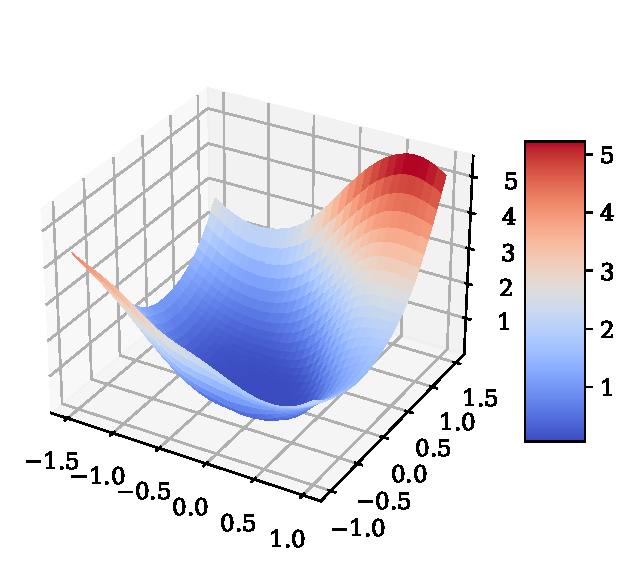
\includegraphics[width=\textwidth,height=2.5cm]{figures/3d_landscape_wiki_tgat_tgn_mixer/wiki_landscape_mixer_surf_file.h5_train_loss_3dsurface.pdf}
    \vspace{-6.5mm}
    \caption{GraphMixer on Wiki}\label{fig:landscape_3d_wiki_tgat_tgn_our_a}
\end{subfigure}
\hspace{0cm}
\begin{subfigure}{0.32\textwidth}
    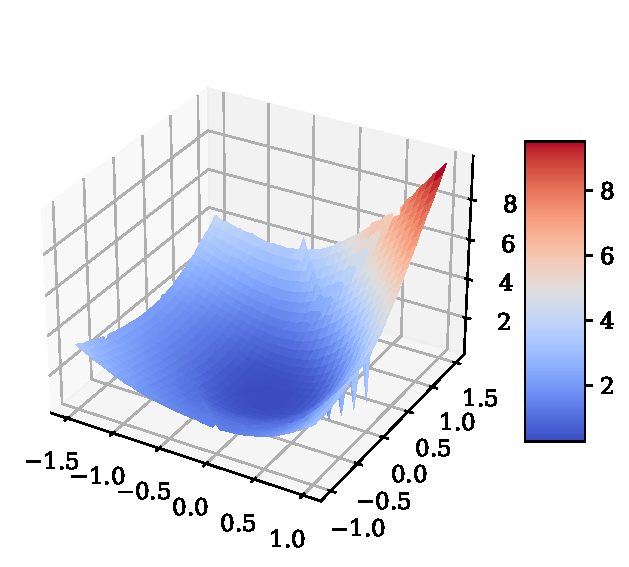
\includegraphics[width=\textwidth,height=2.5cm]{figures/3d_landscape_wiki_tgat_tgn_mixer/wiki_landscape_wiki_tgat_surf_file.h5_train_loss_3dsurface.pdf}
    \vspace{-6.5mm}
    \caption{TGAT on Wiki}\label{fig:landscape_3d_wiki_tgat_tgn_our_b}
\end{subfigure}
\hspace{0cm}
\begin{subfigure}{0.32\textwidth}
    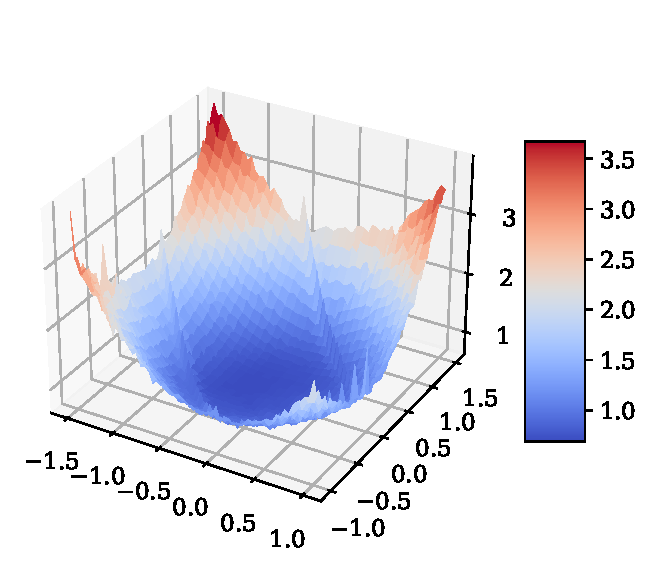
\includegraphics[width=\textwidth,height=2.5cm]{figures/3d_landscape_wiki_tgat_tgn_mixer/wiki_landscape_wiki_tgn_surf_file.h5_train_loss_3dsurface.pdf}
    \vspace{-6.5mm}
    \caption{TGN on Wiki}\label{fig:landscape_3d_wiki_tgat_tgn_our_c}
\end{subfigure}
\begin{subfigure}{0.32\textwidth}
    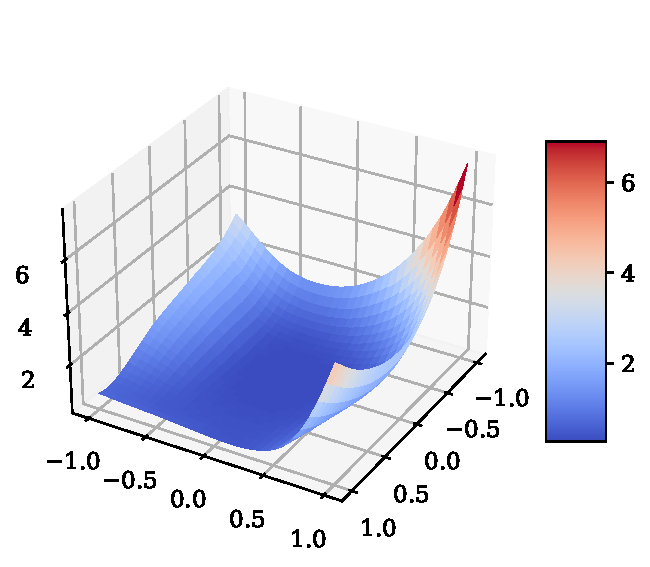
\includegraphics[width=\textwidth,height=2.5cm]{figures/3d_landscape_wiki_tgat_tgn_mixer/gdelt_lite_node_landscape_mixer_surf_file.h5_train_loss_3dsurface.pdf}
    \vspace{-6.5mm}
    \caption{GraphMixer on GDELT-e}\label{fig:landscape_3d_wiki_tgat_tgn_our_d}
\end{subfigure}
\hspace{0cm}
\begin{subfigure}{0.32\textwidth}
    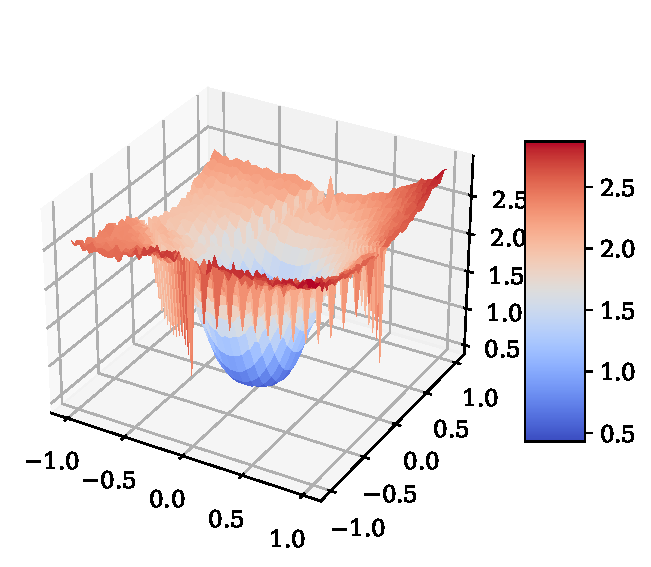
\includegraphics[width=\textwidth,height=2.5cm]{figures/3d_landscape_wiki_tgat_tgn_mixer/gdelt_lite_node_landscape_gdelt_lite_node_tgat_surf_file.h5_train_loss_3dsurface.pdf}
    \vspace{-6.5mm}
    \caption{TGAT on GDELT-e}\label{fig:landscape_3d_wiki_tgat_tgn_our_e}
\end{subfigure}
\hspace{0cm}
\begin{subfigure}{0.32\textwidth}
    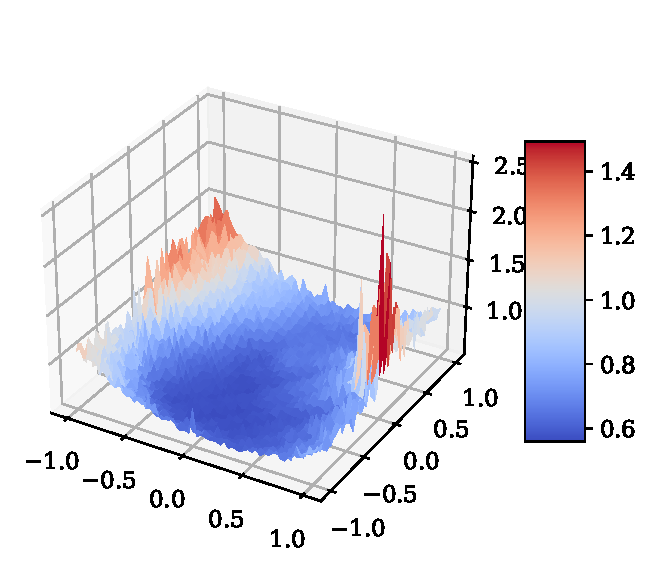
\includegraphics[width=\textwidth,height=2.5cm]{figures/3d_landscape_wiki_tgat_tgn_mixer/gdelt_lite_node_landscape_gdelt_lite_node_tgn_surf_file.h5_train_loss_3dsurface.pdf}
    \vspace{-6.5mm}
    \caption{TGN on GDELT-e}\label{fig:landscape_3d_wiki_tgat_tgn_our_f}
\end{subfigure}
\vspace{-3mm}
\caption{Comparison on the training loss landscape. Results on other datasets and other baselines can be found in Appendix~\ref{section:loss_landscape_appendix}. }
\label{fig:landscape_3d_wiki_tgat_tgn_our}
\vspace{-3mm}
\end{figure}

\noindent\textbf{\our enjoys a smoother loss landscape.}
To understand why \emph{``\our converges faster and generalizes better, while baselines suffer training unstable issue and generalize poorly''}, we explore the loss landscape by using the visualization tools introduced in~\cite{visualloss}.
We illustrate the loss landscape in Figure~\ref{fig:landscape_3d_wiki_tgat_tgn_our} by calculating and visualizing the loss surface along two random directions near the pre-trained optimal parameters. The x- and y-axis indicate how much the optimal solution is stretched along the two random directions, and the optimal point is when x- and y-axis are zero.
\circled{1} From Figure~\ref{fig:landscape_3d_wiki_tgat_tgn_our_a},~\ref{fig:landscape_3d_wiki_tgat_tgn_our_d}, we know \our enjoys a smoother landscape with a flatter surface at the optimal point, the slope becomes steeper when stretching along the two random directions. The steeper slope on the periphery explains why \our could converge fast, the flatter surface at the optimal point explains why it could generalize well.
\circled{2} Surprisingly, we find that baselines have a non-smooth landscape with many spikes on its surface from Figure~\ref{fig:landscape_3d_wiki_tgat_tgn_our_b},~\ref{fig:landscape_3d_wiki_tgat_tgn_our_c},~\ref{fig:landscape_3d_wiki_tgat_tgn_our_e},~\ref{fig:landscape_3d_wiki_tgat_tgn_our_f}. This observation provides sufficient explanation on the training instability and poor generalization issue of baselines as shown in Figure~\ref{fig:train_extra_wiki_lastfm_gdelt_ne},~\ref{fig:train_extra_reddit_mooc_gdelt_e}. Interestingly, as we will show later in Section~\ref{section:time_encoder}, the trainable time-encoding function in baselines is the key to this non-smooth landscape issue. Replacing it with our fixed time-encoding function could flatten the landscape and boost their model performance.


